\documentclass[11pt,a4paper]{article}
\usepackage[utf8]{inputenc}
\usepackage[T1]{fontenc}
\usepackage[brazil]{babel}
\usepackage{lmodern}
\usepackage[margin=2cm]{geometry}
\usepackage{amsmath,amssymb}
\usepackage{booktabs}
\usepackage{graphicx}
\usepackage{hyperref}
\usepackage{xcolor}
\usepackage{titlesec}
\usepackage{tabularx}
\usepackage[section]{placeins}
\usepackage{float}

\hypersetup{
    colorlinks=true,
    linkcolor=blue!70!black,
    citecolor=blue!70!black,
    urlcolor=blue!70!black
}

\titleformat{\section}{\large\bfseries}{\thesection.}{0.5em}{}
\titleformat{\subsection}{\normalsize\bfseries}{\thesubsection.}{0.5em}{}
\titlespacing*{\section}{0pt}{1.2ex plus 0.5ex minus .2ex}{0.6ex}
\titlespacing*{\subsection}{0pt}{1.0ex plus 0.4ex minus .2ex}{0.4ex}

\setlength{\parskip}{0.45em}
\setlength{\parindent}{0pt}

\begin{document}

\begin{center}
    {\LARGE \textbf{Projeto 1: Regressão com MLP e Estudo de Ablação}} \\[0.35em]
    {\large Disciplina: Introdução às Redes Neurais Artificiais} \\[0.3em]
    \textbf{Autor:} Arthur Santos de Oliveira (RA: 156297) \\[0.2em]
    \textbf{Repositório / Código Reprodutível:} \url{https://github.com/Arthur-so/introducao-a-redes-neurais}
\end{center}
\vspace{-0.5em}
\hrule
\vspace{0.8em}

\section{Configuração Experimental}

\subsection{Pré-processamento e Partição dos Dados}

O conjunto possui 300 pares $(x, y)$, com $x \in [0, 10]$ e $y \in [-1{,}49;\ 2{,}66]$. A partição seguiu a proporção exigida: \textbf{10\% treino (30 pontos)}, \textbf{10\% validação (30 pontos)} e \textbf{80\% teste (240 pontos)}, com semente fixa (42) para que a divisão seja sempre a mesma.

Os valores de $x$ e $y$ foram \textbf{padronizados} (média zero e desvio unitário), pois sem isso o SGD puro converge muito lentamente. A média e o desvio foram calculados \textbf{apenas com os dados de treino} e depois aplicados à validação e ao teste, evitando vazamento de informação. Todas as métricas deste relatório estão na escala original de $y$.

\textbf{Referências de desempenho.} Um MSE isolado não diz se o resultado é bom. Por isso, antes de treinar o \textit{baseline}, mediram-se três referências no conjunto de teste (Tabela~\ref{tab:referencias}). O otimizador Adam foi usado apenas nessas medições auxiliares, nunca nos modelos do trabalho.

\begin{table}[h]
\centering
\small
\caption{Referências de desempenho no conjunto de teste.}
\label{tab:referencias}
\begin{tabularx}{\textwidth}{XcX}
\toprule
\textbf{Referência} & \textbf{MSE} & \textbf{Significado} \\
\midrule
Prever sempre a média do treino & 0,518 & Modelo trivial, que ignora $x$ \\
Rede grande + Adam, apenas os 30 pontos de treino & 0,355 & Melhor resultado esperado com tão poucos dados \\
Rede grande + Adam, todos os 300 pontos & 0,142 & Ruído dos dados: nenhum modelo fica abaixo disso \\
\bottomrule
\end{tabularx}
\end{table}

A última linha mostra que, mesmo vendo todos os dados, sobra um erro: é ruído aleatório, impossível de prever a partir de $x$. Portanto, neste problema, o $R^2$ nunca chegaria a 1.

\subsection{Definição e Otimização Empírica do Modelo Baseline (Vanilla)}

O \textit{baseline} é uma MLP básica treinada com \textbf{SGD padrão}, sem Adam, sem \textit{momentum} e sem regularização (L1, L2, \textit{dropout}). O \textit{early stopping} também foi excluído, por ser uma forma de regularização: o modelo final usa os pesos da \textbf{última época}, com número de épocas fixo e igual para todas as configurações.

A busca empírica foi feita em \textbf{três etapas}, sempre escolhendo pelo \textbf{menor erro na validação} (o teste não foi usado em nenhuma escolha): (1) número de camadas e de neurônios; (2) formato das camadas; (3) função de ativação, taxa de aprendizado, tamanho de lote e número de épocas. Em cada etapa, os hiperparâmetros das outras etapas ficaram fixos. A Tabela~\ref{tab:baseline_hiper} resume os valores testados e a configuração escolhida.

\begin{table}[H]
\centering
\small
\caption{Valores explorados e configuração final do \textit{baseline}.}
\label{tab:baseline_hiper}
\begin{tabularx}{\textwidth}{lXl}
\toprule
\textbf{Hiperparâmetro} & \textbf{Valores explorados} & \textbf{Escolhido} \\
\midrule
Camadas ocultas & 1, 2 e 3 & 3 \\
Neurônios por camada & 4, 8, 16, 32, 64 e 128 & 64 \\
Formato das camadas & Uniforme, afunilado, expansivo, gargalo & Uniforme (64-64-64) \\
Função de ativação & ReLU, Tanh & ReLU \\
Otimizador & SGD padrão (sem \textit{momentum} e sem regularização) & SGD \\
Taxa de aprendizado & 0,01; 0,03; 0,1; 0,3 & 0,01 \\
Tamanho do lote & 8, 16, 30 & 8 \\
Número de épocas & 5.000 a 30.000 & 10.000 \\
Função de custo & Erro quadrático médio (MSE) & MSE \\
\bottomrule
\end{tabularx}
\end{table}

O modelo final possui \textbf{8.513 parâmetros}.

\textbf{Repetições.} Os pesos iniciais da rede são sorteados, e esse sorteio muda bastante o resultado: o mesmo \textit{baseline}, trocando apenas a semente, teve erro de validação entre 0,326 e 0,361 --- uma variação de 11\%, maior do que várias das diferenças que queríamos medir. Por isso, \textbf{cada configuração foi treinada três vezes} (sementes 0, 1 e 2, as mesmas para todas as configurações) e reporta-se a média. Quando a diferença entre dois modelos é menor que essa variação entre repetições, eles são considerados \textbf{empatados}. Nas escolhas mais importantes, como a arquitetura, foram usadas 8 repetições.

\textbf{Etapa 1 --- Arquitetura.} As cinco melhores arquiteturas estão na Tabela~\ref{tab:arquiteturas}. As três primeiras ficaram empatadas: as diferenças entre elas são menores que a variação entre repetições. Escolheu-se a \textbf{64$\times$3} por ter a \textbf{menor variação entre repetições no teste} (ou seja, ser a mais estável) e por ter tamanho intermediário.

\begin{table}[h]
\centering
\small
\caption{Melhores arquiteturas (média $\pm$ variação entre 8 repetições). Nesta etapa os demais hiperparâmetros ainda estavam fixos (Tanh, taxa 0,1, lote 16), por isso os valores diferem do resultado final.}
\label{tab:arquiteturas}
\begin{tabular}{lccc}
\toprule
\textbf{Arquitetura} & \textbf{Parâmetros} & \textbf{MSE validação} & \textbf{MSE teste} \\
\midrule
128$\times$3 & 33.409 & $0{,}380 \pm 0{,}032$ & $0{,}377 \pm 0{,}033$ \\
8$\times$2 & 97 & $0{,}396 \pm 0{,}026$ & $0{,}404 \pm 0{,}034$ \\
\textbf{64$\times$3} & \textbf{8.513} & $\mathbf{0{,}405 \pm 0{,}052}$ & $\mathbf{0{,}377 \pm 0{,}013}$ \\
16$\times$3 & 593 & $0{,}436 \pm 0{,}052$ & $0{,}384 \pm 0{,}043$ \\
32$\times$3 & 2.209 & $0{,}457 \pm 0{,}034$ & $0{,}407 \pm 0{,}036$ \\
\bottomrule
\end{tabular}
\end{table}

\textbf{Etapa 2 --- Formato das camadas.} Além de camadas com o mesmo número de neurônios, testaram-se formatos afunilados (ex.: 128-64-32), expansivos (ex.: 32-64-128) e com gargalo (64-16-64). O formato uniforme empatou com o melhor deles, e os formatos afunilados foram os piores.

\textbf{Etapa 3 --- Ativação, taxa, lote e épocas.} A \textbf{ReLU} teve erro menor que a Tanh (0,354 contra 0,373 na validação) e variou cerca de três vezes menos entre repetições. A melhor combinação foi \textbf{taxa 0,01 com lote 8}. Quanto às épocas, o erro de validação diminui até certo ponto e depois volta a subir, porque o modelo passa a decorar o treino (Tabela~\ref{tab:epocas}). O menor erro ocorreu em \textbf{10.000 épocas}.

\begin{table}[h]
\centering
\small
\caption{Erro de validação (MSE) por número de épocas, para a configuração final.}
\label{tab:epocas}
\begin{tabular}{cccccc}
\toprule
\textbf{5.000} & \textbf{10.000} & \textbf{15.000} & \textbf{20.000} & \textbf{25.000} & \textbf{30.000} \\
\midrule
0,397 & \textbf{0,344} & 0,351 & 0,368 & 0,383 & 0,386 \\
\bottomrule
\end{tabular}
\end{table}

\textbf{Resultado do baseline.} A Tabela~\ref{tab:baseline_final} mostra os erros de treino, validação e teste do modelo escolhido (uma execução, semente 0).

\begin{table}[h]
\centering
\small
\caption{Métricas do \textit{baseline} final.}
\label{tab:baseline_final}
\begin{tabular}{lcccc}
\toprule
\textbf{Conjunto} & \textbf{MAE} & \textbf{MSE} & \textbf{RMSE} & \textbf{$R^2$} \\
\midrule
Treino & 0,168 & 0,058 & 0,241 & 0,843 \\
Validação & 0,479 & 0,334 & 0,578 & 0,565 \\
Teste & 0,466 & 0,367 & 0,606 & 0,288 \\
\bottomrule
\end{tabular}
\end{table}

O erro no treino é muito menor que na validação e no teste, o que indica \textbf{sobreajuste}: a rede aprende bem os 30 pontos de treino, mas generaliza pior. (O $R^2$ da validação parece melhor que o do teste porque cada conjunto tem uma dispersão diferente; em MSE, os dois são parecidos.)

\section{Dinâmica de Treinamento e Convergência}

\begin{figure}[h]
\centering
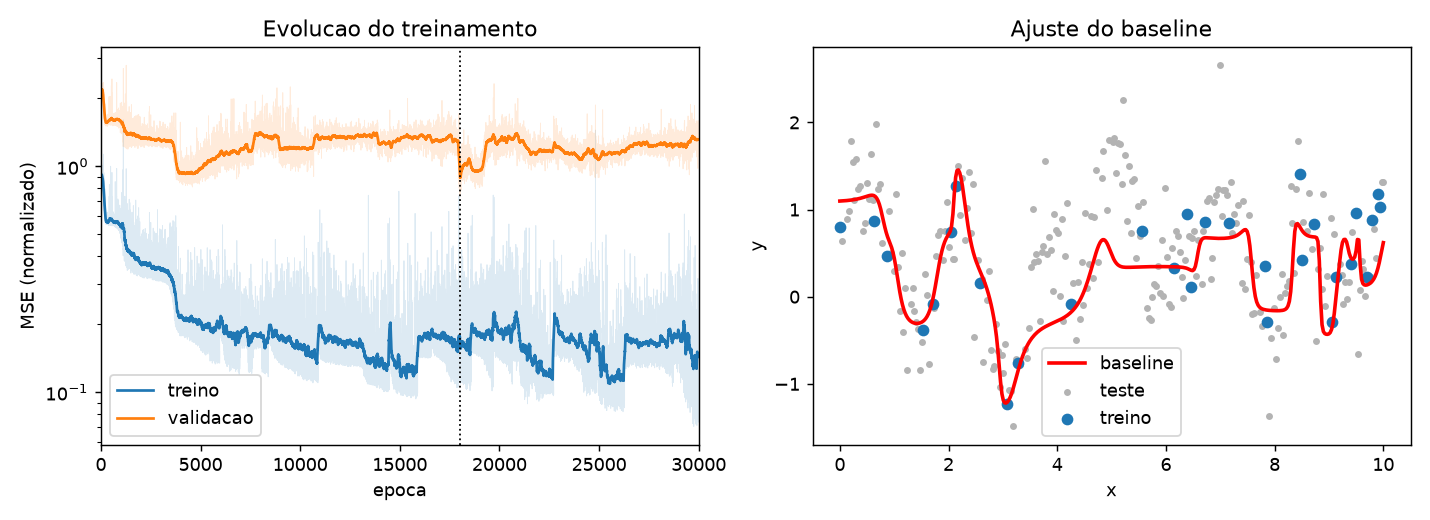
\includegraphics[width=\textwidth]{baseline.png}
\caption{Esquerda: erro de treino e validação do \textit{baseline} ao longo das épocas (escala padronizada). Direita: curva aprendida sobre os dados de teste.}
\label{fig:loss_baseline}
\end{figure}

\begin{itemize}
    \item \textbf{Estabilidade do SGD:} as curvas oscilam bastante porque cada atualização usa apenas 8 amostras. Taxas de aprendizado altas (0,3) fizeram o treino divergir; com 0,01 o treino foi estável.
    \item \textbf{Sobreajuste:} a partir de cerca de 4.000 épocas, o erro de treino continua caindo enquanto o de validação fica estável. A diferença entre os dois é visível na Figura~\ref{fig:loss_baseline}.
    \item \textbf{Momentum:} acelerou bastante a convergência --- com $\beta = 0{,}9$ foram necessárias cerca de 2.900 épocas, contra 7.900 do \textit{baseline} (64\% menos) ---, mas o erro final foi praticamente o mesmo (Figura~\ref{fig:loss_ablation}).
\end{itemize}

\begin{figure}[h]
\centering
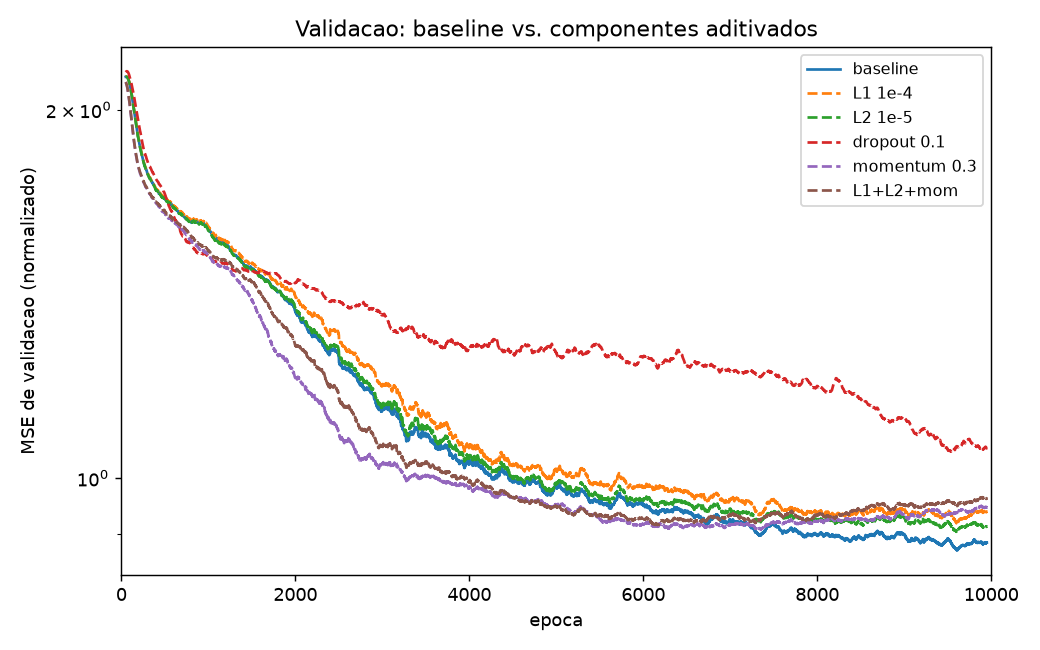
\includegraphics[width=0.8\textwidth]{ablacao_comparacao_64x3_10000.png}
\caption{Erro de validação do \textit{baseline} comparado aos modelos com componentes adicionais.}
\label{fig:loss_ablation}
\end{figure}

\section{Estudo de Ablação e Desempenho no Conjunto de Teste}

Cada componente foi adicionado ao \textit{baseline} sem mudar sua arquitetura, usando as mesmas sementes. Para cada componente, testaram-se diferentes intensidades, e também combinações dos melhores. A Tabela~\ref{tab:ablation_metrics} mostra os resultados no teste (média de 3 repetições).

\begin{table}[h]
\centering
\small
\caption{Estudo de ablação no conjunto de teste (média de 3 repetições). ``Épocas até convergir'' indica quando o erro de validação se estabiliza.}
\label{tab:ablation_metrics}
\begin{tabularx}{\textwidth}{Xccccc}
\toprule
\textbf{Modelo} & \textbf{MSE} & \textbf{RMSE} & \textbf{MAE} & \textbf{$R^2$} & \textbf{Épocas até convergir} \\
\midrule
\textbf{Baseline (SGD sem momentum)} & \textbf{0,3527} & \textbf{0,5938} & \textbf{0,4620} & \textbf{0,3158} & 7.939 \\
\midrule
L1 ($\lambda = 10^{-5}$) & 0,3559 & 0,5964 & 0,4644 & 0,3096 & 7.501 \\
L1 ($\lambda = 10^{-4}$) & 0,3520 & 0,5930 & 0,4614 & 0,3171 & 7.267 \\
L1 ($\lambda = 10^{-3}$) & 0,3844 & 0,6197 & 0,4900 & 0,2543 & 7.865 \\
L2 ($\lambda = 10^{-5}$) & 0,3553 & 0,5959 & 0,4642 & 0,3107 & 7.418 \\
L2 ($\lambda = 10^{-4}$) & 0,3569 & 0,5972 & 0,4648 & 0,3078 & 7.346 \\
L2 ($\lambda = 10^{-3}$) & 0,3590 & 0,5990 & 0,4673 & 0,3036 & 7.695 \\
L2 ($\lambda = 10^{-2}$) & 0,4503 & 0,6710 & 0,5295 & 0,1265 & 7.281 \\
Dropout ($p = 0{,}1$) & 0,3943 & 0,6277 & 0,5006 & 0,2351 & 8.959 \\
Dropout ($p = 0{,}2$) & 0,4081 & 0,6386 & 0,5115 & 0,2083 & 7.655 \\
Dropout ($p = 0{,}3$) & 0,4386 & 0,6622 & 0,5347 & 0,1492 & 7.231 \\
Momentum ($\beta = 0{,}3$) & 0,3534 & 0,5944 & 0,4624 & 0,3144 & 6.369 \\
Momentum ($\beta = 0{,}5$) & 0,3571 & 0,5975 & 0,4650 & 0,3073 & 4.201 \\
Momentum ($\beta = 0{,}7$) & 0,3603 & 0,6001 & 0,4629 & 0,3010 & 5.087 \\
Momentum ($\beta = 0{,}9$) & 0,3588 & 0,5989 & 0,4638 & 0,3040 & 2.884 \\
L2 + momentum & 0,3556 & 0,5962 & 0,4638 & 0,3102 & 5.789 \\
L1 + momentum & 0,3645 & 0,6036 & 0,4690 & 0,2930 & 5.373 \\
L1 + L2 & 0,3573 & 0,5975 & 0,4662 & 0,3069 & 7.716 \\
L1 + L2 + momentum & 0,3648 & 0,6039 & 0,4693 & 0,2924 & 5.124 \\
\bottomrule
\end{tabularx}
\end{table}

\textbf{Nenhum componente melhorou o \textit{baseline}.} O melhor resultado (L1 com $\lambda = 10^{-4}$) reduziu o MSE em apenas 0,0007, valor muito menor que a variação entre repetições. As combinações também não ajudaram. No conjunto de validação, o \textit{baseline} teve o menor erro de todos (0,349).

\textbf{Por quê.} O número de épocas do \textit{baseline} foi escolhido exatamente no ponto de menor erro de validação. Com isso, ele já está no equilíbrio entre aprender pouco e decorar o treino, e a regularização, cuja função é justamente evitar que o modelo decore, não tem mais o que corrigir.

\textbf{Por componente:}
\begin{itemize}
    \item \textbf{L1 e L2:} com valores pequenos, quase não mudam nada; com valores grandes, pioram o modelo (L2 com $\lambda = 10^{-2}$ derruba o $R^2$ de 0,32 para 0,13), pois a penalização impede a rede de aprender.
    \item \textbf{Dropout:} piorou o resultado em todas as intensidades, e quanto maior a taxa, pior. Com apenas 30 pontos de treino, desligar neurônios remove informação útil. Ele também converge mais devagar.
    \item \textbf{Momentum:} não mudou o erro final, mas fez o treino convergir muito mais rápido.
\end{itemize}

\begin{figure}[h]
\centering
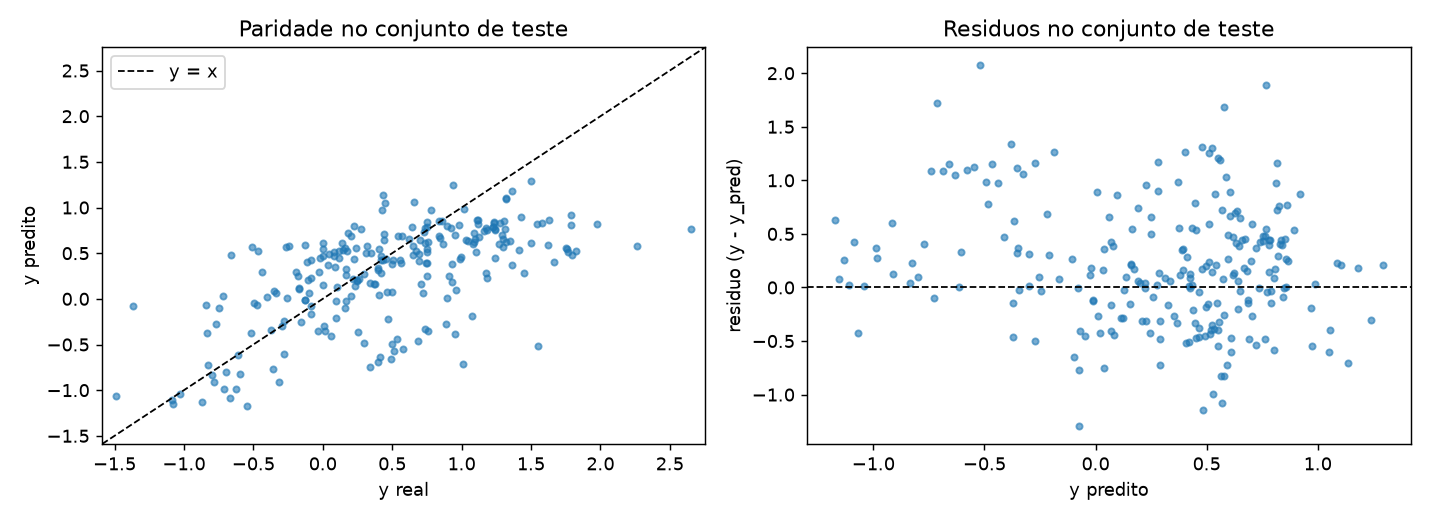
\includegraphics[width=\textwidth]{baseline_residuos.png}
\caption{Esquerda: valor real \textit{versus} previsto no teste (a linha tracejada é a previsão perfeita). Direita: erro de cada previsão.}
\label{fig:parity}
\end{figure}

\textbf{Análise dos erros.} A Figura~\ref{fig:parity} mostra que as previsões ficam \textbf{concentradas perto da média}: o modelo cobre apenas cerca de 60\% da faixa real de $y$ e \textbf{subestima os valores altos}. Com poucos dados e muito ruído, prever perto da média é a forma de errar menos em média, mas isso prejudica os extremos. Nenhum dos componentes testados corrigiu esse comportamento.

\subsection{Estudo Complementar: Rede Maior}

Para verificar se a regularização ajudaria num modelo com mais capacidade, a ablação foi repetida numa rede \textbf{128$\times$3} (33.409 parâmetros, cerca de 4 vezes o \textit{baseline}), mantendo todo o resto igual. Foram testados dois valores de cada componente (Tabela~\ref{tab:complementar}).

\begin{table}[h]
\centering
\small
\caption{Ablação na rede 128$\times$3, no conjunto de teste (média de 3 repetições).}
\label{tab:complementar}
\begin{tabular}{lcc}
\toprule
\textbf{Modelo} & \textbf{MSE} & \textbf{$R^2$} \\
\midrule
\textit{Baseline 64$\times$3 (referência)} & \textit{0,3527} & \textit{0,316} \\
\midrule
\textbf{Rede 128$\times$3 sem componentes} & \textbf{0,3906} & \textbf{0,242} \\
L1 ($\lambda = 10^{-4}$ / $10^{-3}$) & 0,3933 / 0,4185 & 0,237 / 0,188 \\
L2 ($\lambda = 10^{-4}$ / $10^{-3}$) & 0,3852 / 0,3871 & 0,253 / 0,249 \\
Dropout ($p = 0{,}1$ / $0{,}2$) & 0,3892 / 0,4014 & 0,245 / 0,221 \\
Momentum ($\beta = 0{,}5$ / $0{,}9$) & 0,3730 / 0,3702 & 0,276 / 0,282 \\
\bottomrule
\end{tabular}
\end{table}

A rede maior generaliza \textbf{11\% pior} que o \textit{baseline}. Nela, L2, \textit{dropout} leve e \textit{momentum} passam a ter um pequeno efeito positivo, como seria esperado num modelo com capacidade de sobra --- mas as diferenças são pequenas, da mesma ordem da variação entre repetições. E \textbf{nenhuma variante da rede maior superou o \textit{baseline} 64$\times$3}: escolher o tamanho certo da rede foi mais eficaz do que regularizar uma rede grande demais.

\section{Discussão e Conclusões}

\begin{itemize}
    \item \textbf{O limite é a quantidade de dados.} Redes de 97 a 33.409 parâmetros tiveram resultados muito parecidos, e uma rede grande treinada com Adam nos mesmos 30 pontos obteve praticamente o mesmo erro do \textit{baseline} (0,355 contra 0,353). Com 10\% dos dados para treino, nem a arquitetura nem o otimizador mudam muito o resultado.
    \item \textbf{Desempenho realista.} O $R^2$ de teste de 0,288 parece baixo, mas, por causa do ruído dos dados, o máximo possível neste problema é em torno de 0,73. O \textit{baseline} recupera cerca de 44\% do que seria possível aprender.
    \item \textbf{Regularização e momentum.} No \textit{baseline}, nenhuma técnica ajudou, porque o número de épocas já havia sido ajustado no ponto ideal. Numa rede maior, elas passam a ajudar um pouco, mas não compensam o excesso de capacidade. O \textit{momentum} acelera o treino sem melhorar o resultado final.
    \item \textbf{Revisões durante o desenvolvimento.} (i) Uma versão inicial usava \textit{early stopping}; ao removê-lo, por ser uma regularização, toda a escolha de hiperparâmetros foi refeita e mudou. (ii) Inicialmente só se testaram camadas de mesmo tamanho; outros formatos foram testados depois e não foram melhores. (iii) Algumas diferenças que pareciam reais com 3 repetições desapareceram com 8, o que mostrou a importância de repetir os experimentos.
    \item \textbf{Limitações.} A validação tem apenas 30 pontos, o que torna a escolha do modelo sensível ao acaso; a busca foi feita por etapas, e não testando todas as combinações possíveis; e o número fixo de épocas pode prejudicar o \textit{dropout}, que converge mais devagar.
\end{itemize}

\end{document}
